\documentclass[a2,landscape]{a0poster}
\usepackage{mathptmx}
\usepackage[scaled=.90]{helvet}
\usepackage{courier}
\usepackage{postercols}
\usepackage{flowfram}
\setlength{\vcolumnsep}{\baselineskip}
\setlength{\columnsep}{\vcolumnsep}
\Ncolumntop{static}{3}{4in}
\setstaticframe{1}{label={title}}
\newlength\offset
\setlength{\offset}{5in}
\addtolength{\offset}{\vcolumnsep}

%\computeflowframearea{2,3}
%\addtolength{\ffareaheight}{-\offset}
%\setflowframe{2,3}{y=\offset,height=\ffareaheight}
%\newstaticframe{\ffareawidth}{5in}{\ffareax}{0in}[table]

\setstaticframe{2}{clear}
\setallflowframes{border=plain}
\setallstaticframes{border=plain}
\title{Energy-efficient sensing with Android smartphones.}
\author{Martin Maciej Kukla\\
School of Computer Science\\
University of St Andrews
\and
Dr Tristan Henderson\\
School of Computer Science\\
University of St Andrews}
\date{}
\begin{document}
\begin{staticcontents*}{title}
\maketitle
\end{staticcontents*}
\thispagestyle{empty}
\section*{What is a problem?}
\begin{itemize}
   \item Advanced services/ examples
   \item Phone sensing
   \item Energy
   \item Energy-efficient phone sensing
   \item structure: sensor energy measurements + Locy
  \end{itemize}

\mbox{}\framebreak
\section*{What is the solution?}
\subsection*{Sensor energy measurements}
\begin{itemize}
   \item Sample sensor applications
   \item 1\% battery depletion
   \item ?
  \end{itemize}
\subsection*{Locy}
\begin{itemize}
   \item leverage acceleromter
   \item movement detection
   \item adaptive duty-cycling
  \end{itemize}

\mbox{}\framebreak
\section*{Does it work?}
\subsection*{Sensor energy measurements}
\begin{itemize}
   \item complete results
   \item accelerometer versus localization services
  \end{itemize}
  
  \begin{figure}[H]
\centering
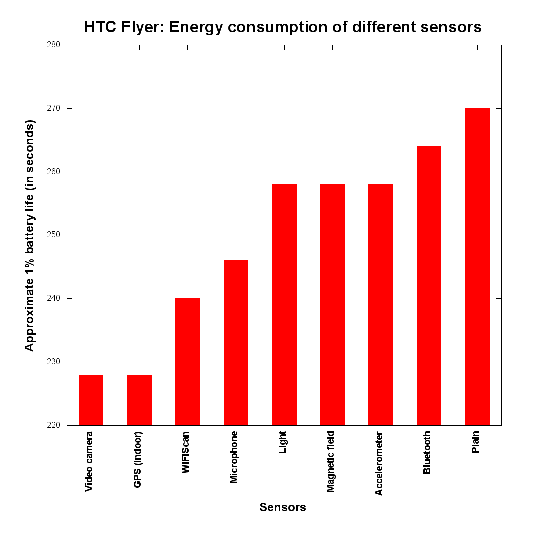
\includegraphics{plots/htc_flyer}
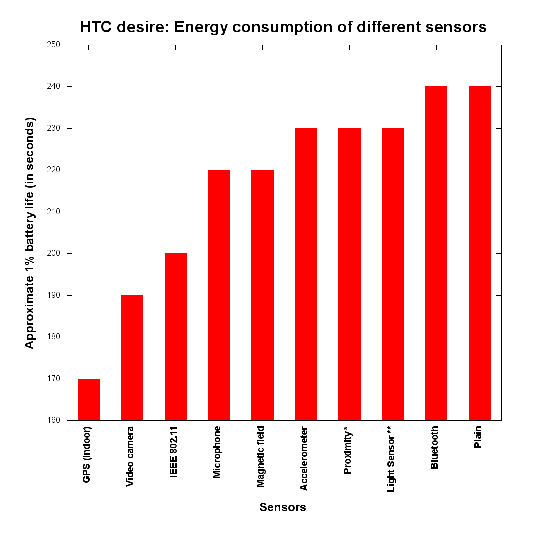
\includegraphics{plots/htc_desire}
%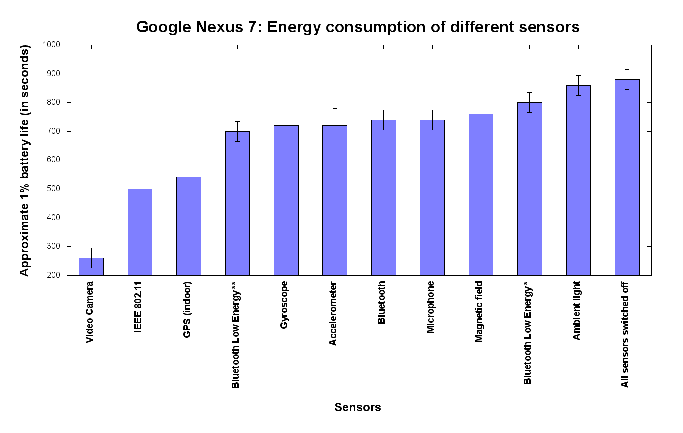
\includegraphics[width=\textwidth, scale=0.9]{plots/google_nexus_7}
\caption{\label{p:all_results} The complete results of energy measurements for all devices. The energy efficiency of different sensors is as expected and overlaps with the results of other research. }
\end{figure}

\begin{figure}[H]
\includegraphics{plots/acc_vs_loc}
\caption{\label{p:all_results} Energy efficiency levels of IEEE 802.11, GPS and accelerometer sensors across different devices. Acceleromter is more energy-efficient, but the difference is not substantial, and thus, efficient accelerometer sampling strategies needs to be introduced. }
\end{figure}

\subsection*{Locy}
\begin{itemize}
   \item energy efficiency performance, different scenarios, different mobile phones
  \end{itemize}
\mbox{}


\end{document}
